\documentclass[../main.tex]{subfiles}

\begin{document}

\section{Electrolytes}
\subsection{Introduction}% and historical context}
Some of the important challenges for development of Li-ion rechargeable batteries for electric vehicles are development of a non-flammable safe electrolyte with large operating voltage window that can develop rapidly a SEI layer to prevent plating of Li on a carbon anode and allows fast charging of the battery.\cite{Goodenough2010} Figure \ref{fig:electrolyte} schematically shows the electronic energy levels in electrode and electrolyte of a battery cell. An anode with an electrochemical potential $\mu_{A}$ above the lowest unoccupied molecular orbital (LUMO) of the electrolyte will reduce the electrolyte unless a passivation layer creates a barrier to electron transfer from the anode to the electrolyte LUMO. Similarly, a cathode with a $\mu_{C}$ below the highest occupied molecular orbital (HOMO) will oxidize the electrolyte unless a passivation layer blocks electron transfer from the electrolyte HOMO to the cathode. Therefore, the electrochemical potentials $\mu_{A}$ and $\mu_{C}$ should lie within the the energy separation E$_g$ of the LUMO and the HOMO of the electrolyte, which constrains the open-circuit voltage $V_{\rm oc}$ of a battery cell:
\begin{equation}
    eV_{\rm oc}=\mu_{A}-\mu_{C}\leq E_{g}
\end{equation}
where $e$ is the magnitude of the electron charge. %A passivating SEI layer at the electrode/electrolyte boundary can give a kinetic stability to a larger $V_{\rm oc}$ provided that $eV_{\rm oc}-E_{g}$ is small. 
The formation of the SEI layer comes with the cost of irreversible capacity loss.
\begin{figure}
    \centering
    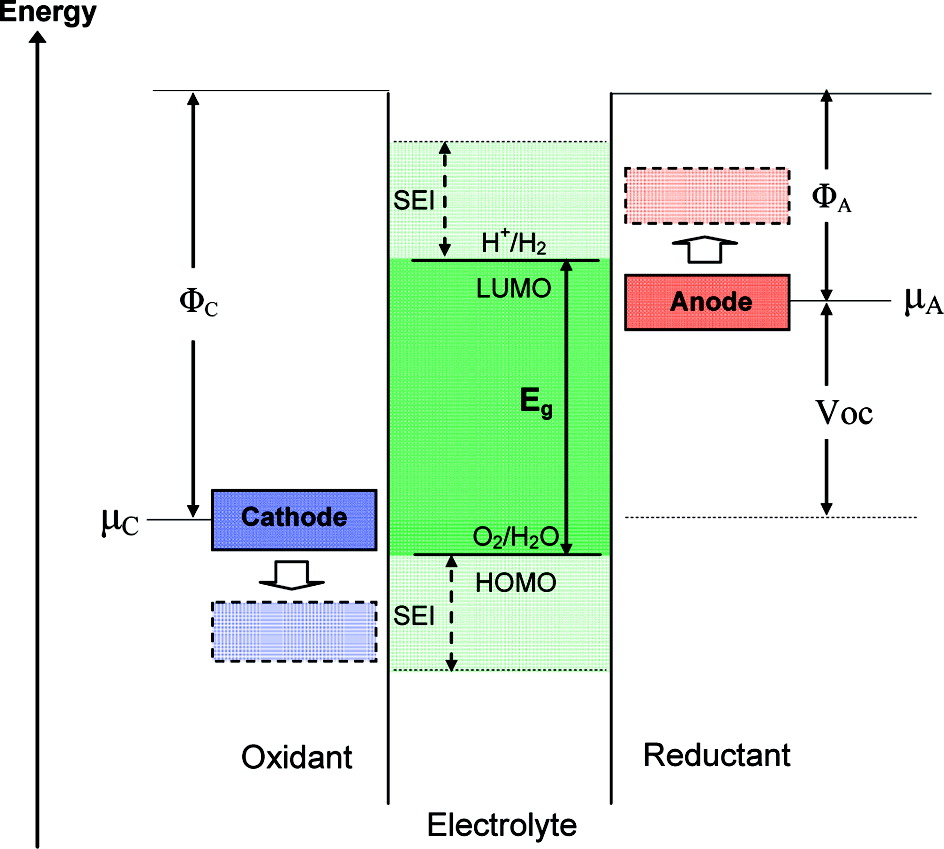
\includegraphics{figures/electrolyte.jpeg}
    \caption{Schematic open-circuit energy diagram of an aqueous electrolyte. $\Phi_{A}$ and $\Phi_{C}$ are the anode and cathode work functions. $E_{g}$ is the window of the electrolyte for thermodynamic stability. A $\mu_{A}>$ LUMO and/or a $\mu_{C}<$ HOMO requires a kinetic stability by the formation of SEI layer. Reproduced from Ref. \citenum{Goodenough2010} }
    \label{fig:electrolyte}
\end{figure}


For an aqueous electrolyte $E_g \approx 1.3 $  eV  limits the $V_{oc}$. In order to obtain a cell with a higher $V_{oc}$ and therefore a higher energy density, it is necessary to turn to a non-aqueous electrolyte with a larger $E_g$. This observation, in turn, has led to the Li-ion battery since lithium salts are soluble in some non-aqueous solvents and polymers.

Apart from larger thermodynamic stability window, another requirement is high ionic conductivity ($>10^{-4}$ S/cm) in the electrolyte and across the electrode-electrolyte interface for a high rate-capability. Figure \ref{fig:conductivity} shows the ionic conductivities of common non-aqueous  electrolytes.\cite{Kamaya2011} These can be broadly classified into liquid and solid electrolytes. In the next subsections, we describe some of the liquid and solid electrolytes, their ionic diffusivity and stability. 

\begin{figure}[htbp]
    \centering
    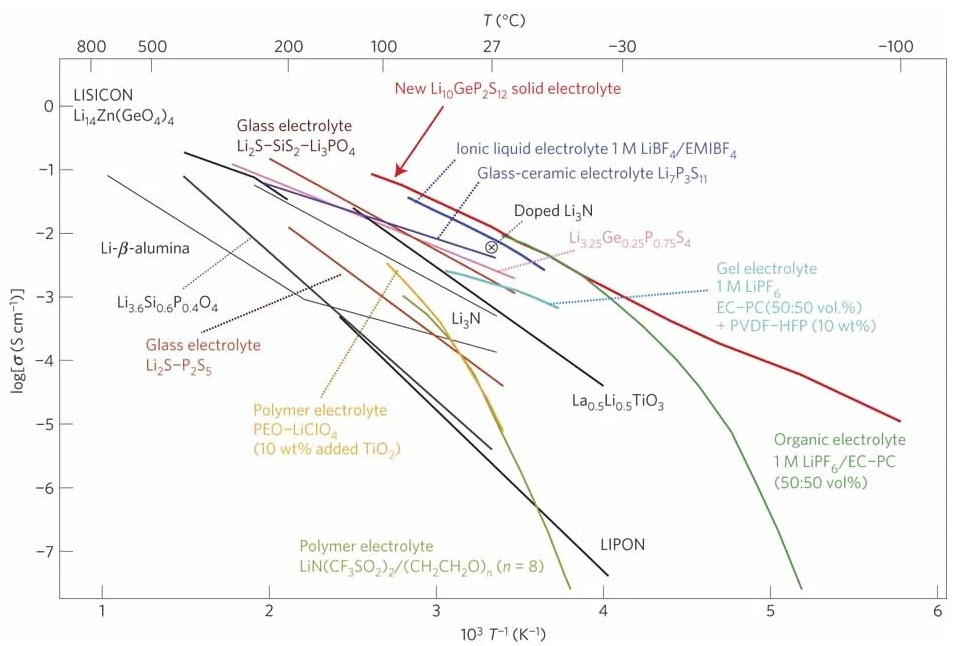
\includegraphics[scale=0.6]{figures/conductivity.jpg}
    \caption{Ionic conductivity of different electrolytes, reproduced with permissions from Ref. \citenum{Kamaya2011}}
    \label{fig:conductivity}
\end{figure}

%General picture and types of electrolytes. The importance of moving from liquid to solids and the challenges involved.
%General description, broad picture.
%Compatibility between electrolyte types and anode/cathode types. In terms of the cathodes, we discuss layered oxides (NMC), layered oxides (LiMn$_2$O$_4$), and polyanions (LiFePO$_4$), so if we can link electrolytes to these specific materials, it would prelude to the cathodes section. Similarly to the anodes section if possible?




\subsection{Liquid Electrolytes (Maxim and Arihant)}
\label{sec:Liquid_electrolytes}
\subsubsection{Introduction (MZ/Arihant)}
%Brief intro to liquid electrolytes, highlighting the importance of atomistic modelling. Introducing widely used liquid electrolytes, mixtures with solvents/common solvents. What materials/properties will be discussed here i.e. used as examples.

%Maybe something about impotance of electrolytes, like:
%Understanding electrolytes is very important in overall electric batteries modeling, as electrolytes may be "bottle-necks" in carrying high current density. may strongly affect degradation mechanisms, thermal effects, etc.

The most widely used liquid electrolyte in Li-ion batteries is LiPF$_6$ in a solvent, which is typically a mix of two or more solvents, for example propylene carbonate (PC), ethylene carbonate (EC), ethyl methyl carbonate (EMC), dimethyl carbonate (DMC), in order to achieve competing objectives such as ability to dissolve high concentration of salt, low viscosity, high dielectric constant, at typical operational temperatures. Cyclic carbonates (EC, PC) have higher dielectric constant but also high viscosity, while ``linear'' carbonates (DMC, EMC) low viscosity but also low dielectric constant; for that reason often mixtures of solvents are used to optimise performance in a specific application are used.

\begin{figure}
    \centering
    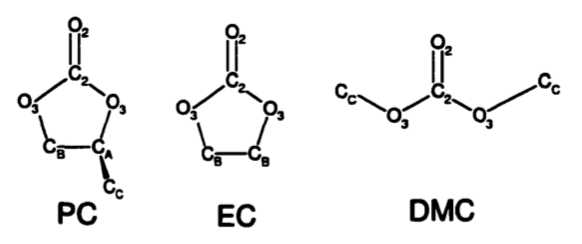
\includegraphics[scale=0.3]{figures/LE1.PNG}
    \caption{Molecular structure for solvents: propylene carbonate (PC), ethylene carbonate (EC), dimethyl carbonate (DMC).}
    \label{fig:LE1}
\end{figure}

\subsubsection{Diffusion Coefficients for Continuum Modelling (Maxim/Arihant)}
Atomistic modelling of liquid electrolyte aims to provide valuable insight into the material properties of electrolyte mixtures. However, these models can also assist in the parameterisation of continuum models by providing predictions of atomistic simulations, helping to understand the results of physical experiments, and aid in testing assumptions underpinning continuum modeling.

%start: version 2,  30 January 2021

A widely used approach to continuum modeling of electrolytes is based on concentrated solution theory, pioneered by John Newman \citenum{Newman2004}. A key parameter for determining transport properties of electrolytes are Stefan-Maxwell diffusivities. These can be modelled atomistically, but such simulations are not as widely developed as more traditional approaches such as Green-Kubo. In concentrated solution theory, other electrolyte model parameters including salt diffusivity, transference number,  and apparent conductivity are derived from the Stefan-Maxwell diffusivities and certain thermodynamic parameters (section ~\ref{sec:stefan-maxwell}, Equations.~\ref{cp diff_def} -  ~\ref{mcinn}).

There are other approaches aimed to compute the same physical quantities, for example electric conductivity, from different perspectives, such as by deriving it from mobility coefficient and estimating the latter based on the Stokes law \cite{Gering2017}.

Stefan-Maxwell diffusivities play a key role in continuum modeling of electrolytes, but are not sufficiently studied in the atomistic literature. Here, we pay particular attention to atomistic computations of Stefan-Maxwell diffusivities and related alternative approaches. Exact relationships between different approaches is presently not clear, and we feel it will be great if it is further clarified. % no claim that all related literature is covered

%%added discussion, may need different placement
\noindent {\bf Stefan-Maxwell diffusivities, self-diffusivities, Green-Kubo diffusivities, and continuum modelling}.
As described in section \ref{sec:diffusion}, both the Stefan-Maxwell and Green-Kubo approaches are used in molecular dynamics for calculating diffusion coefficients.  %For this reason, we emphasize below the Stefan-Maxwell approach, and indicate how the quantities computed in this approach can be translated to more traditional Green-Kubo quantities.

The Stefan-Maxwell and Green-Kubo diffusivities are different, both conceptually and in the way they are computed. Stefan-Maxwell diffusivities are relative diffusivities, labeled by a pair of species in a relative motion. Green-Kubo diffusivities are single-labeled by the index of species of the tagged particle being studied. The main advantage of the Stefan-Maxwell approach is that they correctly model forces vs. fluxes relationships of necessarily multi-component dynamics, with all the species, both electrically charged and neutral, moving past each other, not just tracer particles moving independently in a stationary fluid. However, the Green-Kubo approach is better studied and more widely used in the molecular dynamics community for a broad range of materials and is considered standard.

Batteries require high current densities and therefore use concentrated electrolyte solutions. Stefan-Maxwell diffusivities are the most suited for modelling concentrated electrolytes. Such electrolytes may form complicated mixtures of fully and partially dissociated ions, and clusters of ions and solvent molecules traveling together. Concentrated solution theory is based on general thermodynamic considerations and thus is capable of accommodating those possibilities, while modelling assumptions suitable for dilute solutions, for example assuming that particles are moving independently, or that their interactions can be treated within a mean field approximation, require a justification, and need not apply.

Since sizes, geometry, and spatial distribution of charges of $+$ and $-$ ions are not the same, there is no reason for ionic diffusivities $D_+$ and $D_-$ in the Green-Kubo approach to be equal. However, continuum models of electrolytes assume electrolyte electrical neutrality, and operates with a single electrolyte diffusivity $D_e$, not with $+$ and $-$ ionic diffusivities separately. With the Stefan-Maxwell diffusivities, the passage to diffusivity $D_e$ entering the continuum model is immediate, Eq. \ref{cp diff_def}. While with the Green-Kubo ones, identification of $D_+$ with Stefan-Maxwell diffusion coefficient $D_{0+}$  might be a natural first guess, however the issue of how to use ionic diffusivities needs further modeling assumptions, such as Nernst-Plank-Poisson model, which is a mean-field model. For concentrated solutions, such models suffer from difficulties in defining convection and flux terms in the species mass conservation equations.
%Debye-Huckel model in addition uses linearized version of the Poisson-Boltzmann equation, justified for dilute solutions. %Noted, I do not know good references straight away; see eg MIT lectures of Bazant as intiial reference

In the concentrated solution theory framework, all other electrolyte continuum modeling parameters required in the DFN model, conductivity and transference number, are derived from Stefan-Maxwell diffusivities and thermodynamic factors  (see section ~\ref{sec:stefan-maxwell}). In other approaches, the meaning and method of computing the remaining continuum modelling parameters has to be established in addition.

%%end of added discussion

\noindent {\bf Atomistic modelling}
%{\tiny \red there is presently not enough time to compare results of different approaches, or transcribe here further details of those approaches. To consider: adding some of the above, time permitting. MZ.}
%At least conceptually, the best way to compute Stefan-Maxwell diffusivities is via decay of correlations method, based on Onsager's decay of fluctuations hypothesis, and briefly described in section 2.2.2. However, greatest proportion of molecular dynamics literature reports diffusivities computed by  the Green-Kubo mean square displacement method.

The simplest model of electrolyte is a binary electrolyte, comprised of positive and negative ions of lithium salt and composite solvent, with its various constitutive parts at thermodynamic equilibrium. The properties of such an electrolyte will still depend on the solvent composition and salt concentration.


Computation of Stefan-Maxwell diffusivities via the decay of correlations method, based on Onsager's decay of fluctuations hypothesis, and briefly described in section~\ref{sec:stefan-maxwell} for LiPF$_6$ in PC and EC/DMC solvents was performed by \citeauthor{2002PhDWheeler}, using a simple ball-and stick binary electrolyte model for solvent molecules with Lennard-Jones and Coulomb interaction potentials for solvent atoms and LiPF$_6$ ions, \cite{2002PhDWheeler} which are shown in table \ref{tab:wheeler}. Original molecular dynamics code was used in those simulations.

Recently, for PC solvents, a careful experimental measurement of all continuum modeling parameters by \citeauthor{Hou2020} for 1 M salt concentration gave:\cite{Hou2020}
%\begin{equation} \begin{array}{l}
 $ \mathcal{D}_{0+}=  4.5$, $  \mathcal{D}_{0-}= 20.0 $  and $   \mathcal{D}_{+-}=  2.0$ (all in $    10^{-11}$m$^2$/s)
%    \label{FigHouMonroeStMExpPC}
%\end{array} \end{equation}
which are quite close to the computed values by Wheeler.\cite{2002PhDWheeler}
%table Wheeler
\begin{table*}[htbp]
    \caption{Stefan Maxwell binary diffusivities for 1 M LiPF$_6$ in PC and 1:2 w/w EC/DMC from Ref. \citenum{2002PhDWheeler} and corresponding experimental values from Refs. \citenum{Hayamizu1999, Kondo2000, TARASCON1994293, Capiglia1999}. The uncertainty in both computed and experimental values is 30 $\%$.}
    \centering
    \begin{tabular}{|l|r|r|r|r|} \hline
        %\multicolumn{1}{c}
        %{Solvent} &
        \multirow{2}{*}{$\mathcal{D}~(10^{-11}$m$^2$/s)} & \multicolumn{2}{|c|}{PC} & \multicolumn{2}{|c|}{EC/DMC} \\ \cline{2-5}
        & Computed & Experimental & Computed & Experimental \\ \hline
        % PC &
        $\mathcal{D}_{0+}$ & 4.9 & 7.0 & 11.8/20.7 & 9.2/25.3 \\ \hline
        $\mathcal{D}_{0-}$ & 14.3 & 17.1 & 16.6/38.2 & 24.1/31.1\\ \hline
        $\mathcal{D}_{+-}$ & 0.2 & 2.6 & 0.2 & 3.4\\ \hline
    \end{tabular}
    \label{tab:wheeler}
\end{table*}

A different computational approach\cite{rosstaylor1993, Krishna2005,FongTransport2020,Mallarapu2021} to Stefan-Maxwell diffusivities is based on a form of Stefan-Maxwell relations resolved for the fluxes, see section \ref{sec:stefan-maxwell} Eq. ~\ref{StM:L} and following discussion on additional restrictions this pseudo-inverse form has to satisfy. It is proposed by \citeauthor{Krishna2005} to compute Onsager coefficients $L_{ij}$ of the flux-resolved form of Stefan-Maxwell relations in a way similar to the Green-Kubo method of computing diffusion coefficients,\cite{Krishna2005}

\begin{equation} \begin{array}{l}
    \displaystyle L_{ij} = - \frac{1}{6 N} \lim_{\Delta t \rightarrow \infty}
    \left\langle
   \left( \sum_{k=1}^{N_i} \mathbf{r}_{k,i} (t + \Delta t) - \mathbf{r}_{k,i} (t ) \right)
   \left( \sum_{l=1}^{N_j}  \mathbf{r}_{l,j} (t + \Delta t) - \mathbf{r}_{l,j} (t ) \right),
    \right\rangle
    \label{StMGKMD}
\end{array} \end{equation}

\noindent where $i,j$ label species, $k,l$ label molecules of same species,  $\left\{ N_i \right\}$ are number of molecules of each species, $N= \sum_i N_i$ is the total number of molecules. This is an interesting approach which essentially treats the gradient of the chemical potential as a force, and uses all the assumptions of the Green-Kubo method. It will be interesting to have better justification of applicability of those assumptions for concentrated solutions, whose continuum mass transport equations have a convection term, and how is the proposed method affected by the fact that ``forces'' here are not independent while velocities are determined by ``forces'' only up to a reference velocity. Results for the Green-Kubo classical MD self-diffusivities and Stefan-Maxwell diffusivities computed from those using generalized Darken relations can be found in Figures 2, 3 and in the supplementary information of Ref. \citenum{Mallarapu2021}. Simulations for the  LiPF$_6$ with EC/EMC were performed in LAMMPS using antechamber tool for EC and EMC parameters and using a GAFF \cite{Wang2004GAAF} forcefield.

Further, Darken \cite{Darken} relations 
\begin{equation} \begin{array}{l}
    \displaystyle  D_{ij} = y_j D_i + y_i D_j ,
    \label{Darken}
\end{array} \end{equation}
and generalized Darken relationships between Green-Kubo diffusivities $\left\{ D_i \right\}$ and Stefan-Maxwell ones, $\left\{ D_{ij}\right\}$ are proposed \cite{rosstaylor1993,Krishna2005,Mallarapu2021},
\begin{equation} \begin{array}{l}
    \displaystyle  D_{ij} = \frac{y_j}{y_i+y_j} D_i + \frac{y_i}{y_i+y_j} D_j ,
    \label{DarkenGen}
\end{array} \end{equation}
where $\left\{ y_i \right\}$ are molar fractions. Those relations are phenomenological, with some evidence provided by Green-Kubo like computations of Stefan - Maxwell diffusivities\cite{Krishna2005}. Further, a version of Darken relations for EC:EMC mix is proposed, see Eq. 3, 4 in \cite{Mallarapu2021}.

Ab-initio and classical MD, described in section \ref{sec:molecular_dynamics}, can provide information on coordination numbers and solvation mechanisms for different solvents. \cite{Ong2015} The trajectories of solvation structures and Li-P distances for LiPF$_6$ in EC are presented in figure \ref{fig:Ong2015}. The authors used both ab-initio and classical MD, reporting the same solvation structure for both methods.

\begin{figure}
    \centering
    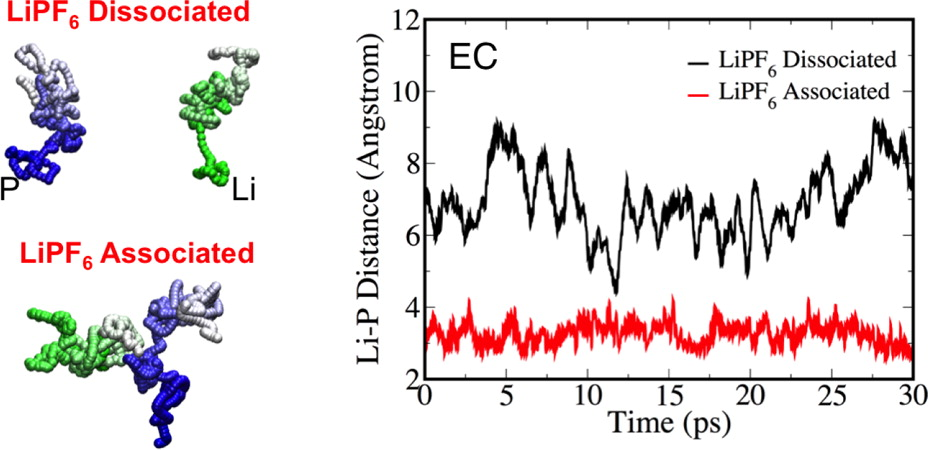
\includegraphics{figures/aimd.jpeg}
    \caption{(Left) Trajectories for Li$^+$ and P atom of PF$^-_6$ for a 63 EC +1 LiPF$_6$ system\cite{Ong2015}. Color designate time, darker colors are earlier in time. (Right) Li-P distance as a function of time for the trajectories.}
    \label{fig:Ong2015}
\end{figure}

It may be challenging to obtain kinetic parameters, such as diffusion coefficients, using first principle methods. For example, the displacement presented in figure \ref{fig:Ong2015} is oscillatory and essentially flat, in both the associated and dissociated cases, and without further study, can only convey information about solvation structure but not diffusion coefficients. \citeauthor{Ong2015} also calculate Green-Kubo diffusion coefficients, presented in table \ref{tab:ong}. DFT simulations were done in the VASP package. MD simulations were performed with ReaxFF force field and using NVT ensemble implemented by Nose-Hoover thermostat.
%figures~\ref{fig:FPMD_Li} and \ref{fig:FPMD_PF6}.

An interesting observation is made in the paper that diffusion coefficients obtained from mean square displacement or velocity autocorrelation methods are not equivalent, unlike is expected in the Green-Kubo framework (see Eq. ~\ref{eq:self-diffusion} - ~\ref{velAC}), likely signalling limitations of the Green-Kubo method. Indeed, the method does not predict crossover time-scales from oscillatory to approximately linear behavior of the mean square displacement, or time scale sufficient for molecular dynamics simulation to predict parameters of the continuum models, operating at much longer time scales then would be practical in a molecular dynamics simulations, especially ab-initio ones.

%Here,  (while it is not immediately clear to us whether diffusion coefficients were significantly affected).

% table goes here
\begin{table*}[htbp]
    \caption{Calculated diffusion coefficients from the slope of mean-square displacement (MSD) and from integral of the velocity autocorrelation function (VACF) from Ref. \citenum{Ong2015}. }
    \centering
    \begin{tabular}{|l|r|r|r|r|}
        \hline
        %\multicolumn{1}{c}
        %{Solvent} &
        \multirow{2}{*}{Electrolyte Composition} & \multicolumn{2}{|c|}{Li$^+$} & \multicolumn{2}{|c|}{PF$^-_6$} \\ \cline{2-5}
        & MSD & VACF & MSD & VACF \\ \hline
        63 EC + 1 LiPF$_6$ & $5.2\pm0.8$ & $7.9\pm1.3$ & $7.1\pm0.9$ & $9.2\pm1.0$ \\ \hline
        42 EMC + 1 LiPF$_6$  & $9.6\pm1.6$ & $10.1\pm2.1$ & $30.8\pm8.8$ & $28.6\pm5.7$ \\ \hline
        15 EC + 35 EMC + 1 LiPF$_6$  & $2.6\pm1.3$ & $5.1\pm1.1$ & $5.7\pm2.4$ & $9.5\pm1.4$ \\ \hline
    \end{tabular}
    \label{tab:ong}
\end{table*}
%table ends here

% \begin{figure}
%     \centering
%     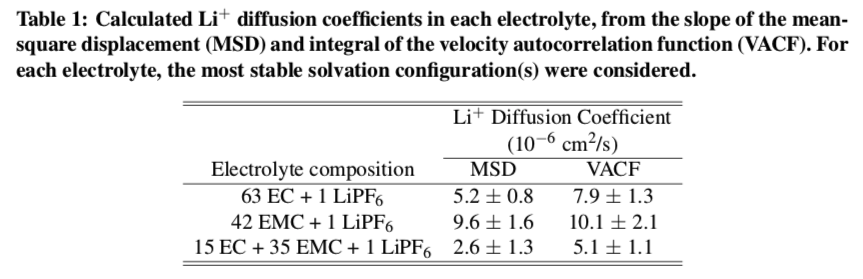
\includegraphics[scale=0.5]{figures/FPMD_Li.png}
%     \caption{}
%     \label{fig:FPMD_Li}
% \end{figure}

% \begin{figure}
%     \centering
%     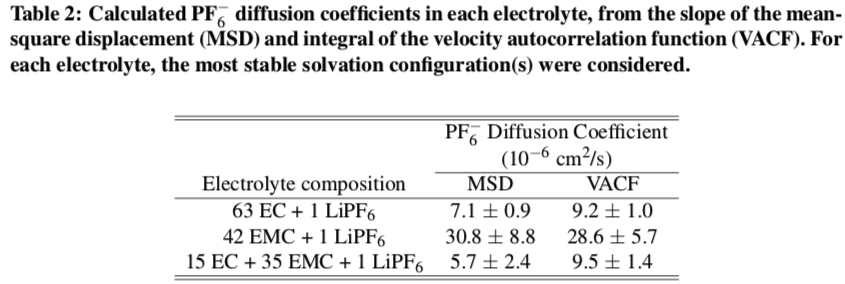
\includegraphics[scale=0.6]{figures/FPMD_PF6_.png}
%     \caption{}
%     \label{fig:FPMD_PF6}
% \end{figure}

A well-developed case of molecular-based methods not using concentrated solution theory is the Advanced Electrolyte Model (AEM)\cite{Gering2006,Gering2017,Logan2018,Dave2019,Logan2020}, developed by \citeauthor{Dave2019} and implemented as a software package.\cite{Dave2019} The AEM approach to computing conductivity uses improved versions of the Stokes' law of drag on a particle in viscous flow, in order to express conductivity via particle mobility. The basic Stokes' law is modified to account for various physical effects in electrolytes. Stokes' drag is corrected to take account for retarding solvent-ion and opposite ion interactions, motion type (hopping or flowing), etc. All the physical factors taken into account are illustrated in Figure 1 in \citenum{Gering2017}. Figure 3, ibid, shows simulation results for conductivity of PC- LiPF$_6$ system at 25$^o$ and concentrations up to 3M, and comparison of simulation with experimental data. The match is quite good, apart from concentrations of 0.4-0.8 M where conductivity reaches maximum and discrepancy of simulation and experiment is about 15\%.

AEM also provides corrections to the viscosity factor in the Stokes' law to account for additional effects, such as non-spherical particle and solvation effects on effective particle size. It starts with baseline viscosity of mixed solvent with no salt, and corrects it by a product of empirical factors. \cite{Gering2006})

AEM modelling results for conductivity and viscosity for LiPF$_6$ in EC:EMC and  EC: DMC, and conductivity for EC:DMC :MA and EC:EMC :MA solvent blends are shown in Figure ~\ref{AEM}.

%uploaded figures and figure captions from the paper. Caption may be shortened, leaving detailed one for now 
\begin{figure}
    \centering
    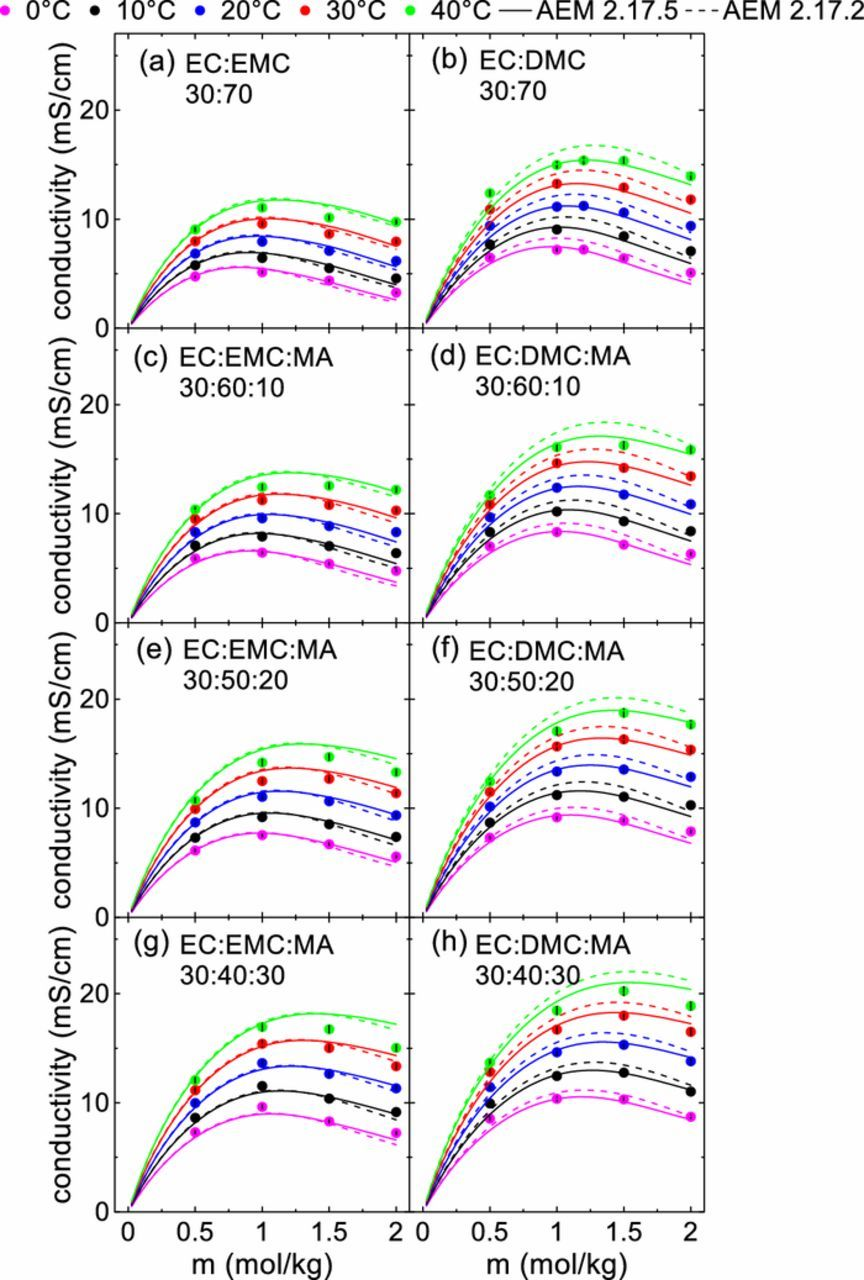
\includegraphics[scale=0.75]{figures/JES 165 Gering 2.jpeg}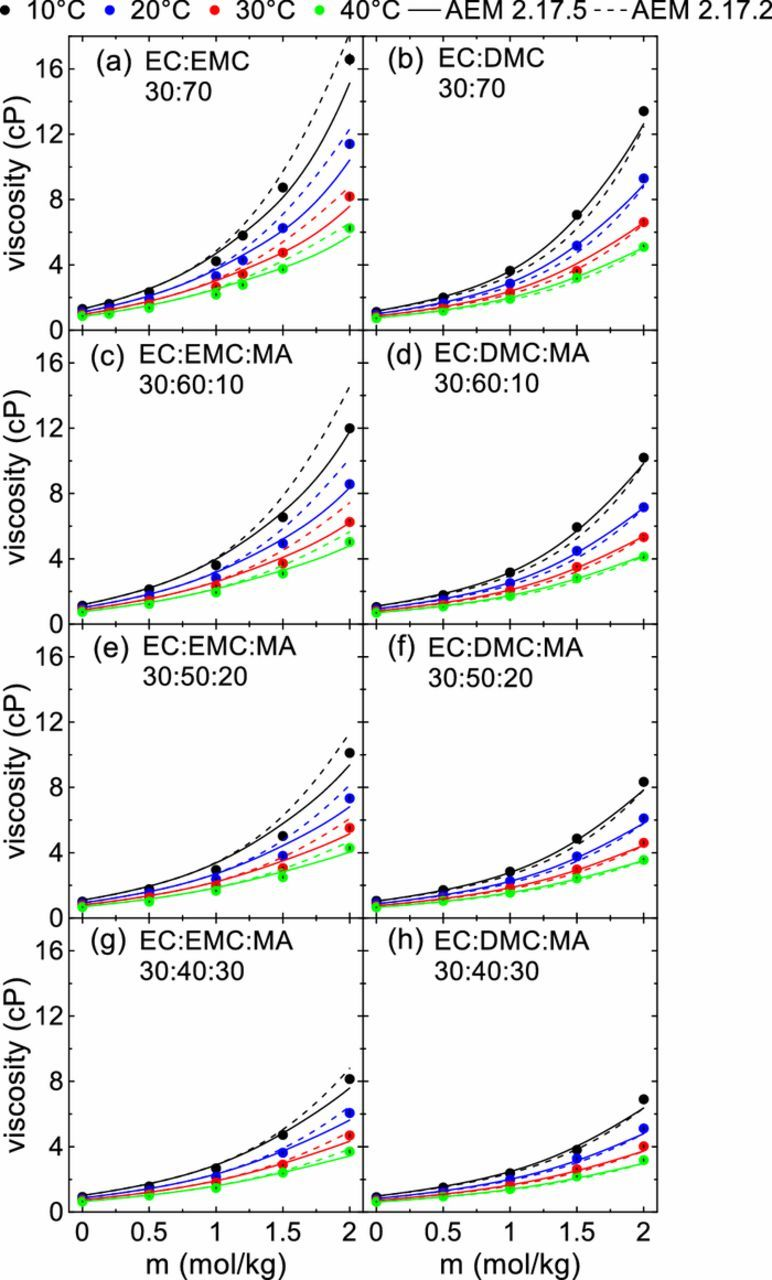
\includegraphics[scale=0.75]{figures/JES 165 Gering 1.jpeg}
    \caption{Left:  Ionic conductivity as a function of  LiPF$_6$ concentration for electrolytes with the solvent blends (a) EC:EMC 30:70, (b) EC:DMC 30:70, (c) EC:EMC:MA 30:60:10, (d) EC:DMC:MA 30:60:10, (e) EC:EMC:MA 30:50:20, (f) EC:DMC:MA 30:50:20, (g) EC:EMC:MA 30:40:30, and (h) EC:DMC:MA 30:40:30, all given in weight percent. Calculations from two different versions of the AEM are shown in solid and dashed lines, for AEM 2.17.5, and AEM 2.17.2, respectively.
    Right: Viscosity as a function of  LiPF$_6$ concentration for electrolytes with the solvent blends (a) EC:EMC 30:70, (b) EC:DMC 30:70, (c) EC:EMC:MA 30:60:10, (d) EC:DMC:MA 30:60:10, (e) EC:EMC:MA 30:50:20, (f) EC:DMC:MA 30:50:20, (g) EC:EMC:MA 30:40:30, and (h) EC:DMC:MA 30:40:30, all given in weight percent. Calculations from two different versions of the AEM are shown in solid and dashed lines, for AEM 2.17.5, and AEM 2.17.2, respectively. These images are reproduced with permissions from ref~.\citenum{Logan2018}.  }
    \label{AEM}
\end{figure}

%AEM, developed as a licensed software package based on an extension of those ideas, can be used to predict properties of electrolytes with different solvent mixes and salt concentrations,\cite{Logan2018,Logan2020} to account of some of the computational results and their comparison with experiments.

Perhaps a drawback of AEM is quite a large number of empirical fitting parameter. Data analysis and fitting methods or machine learning methods may become competitive with such physics-based methods with large number of fitting parameters, and experimental papers measuring electrolyte properties often provide\cite{Hou2020,Wang2020} fitting functions, which may be not be physics-based.

It may be interesting to see whether first-principle methods can assist in predicting or computing fitting parameters introduced in AEM model, especially those which have transparent geometric meaning, such as solvation radius and coordination numbers and volumes.
%end: version 2,  30 January 2021

\subsubsection{Activity coefficients of electrolytes (Arihant)}
%The charge transport in electrolytes is described by their activity coefficients, which 
The activity coefficients of electrolyte can be calculated using DFT+PB simulations of solutes in electrolyte solutions as described in sec.\ref{sec:tf}. A sample calculation of the activity coefficient of LiPF$_6$ in ethylene carbonate solvent is discussed here from Ref. \citenum{Dziedzic2020}. The experimental value of bulk permittivity of ethylene carbonate (EC) is ($\veps^\infty=90.7$)\cite{Hall2015} and the surface tension of EC is (0.0506~N/m),\cite{Naejus2002} which are used for these calculations. %are taken from the literature. 
The solvent radius is set to $R^\textrm{solvent}_k= 10.5~a_0$ to approximate the size of an EC molecule, and the isovalue of solute electronic density ($\denselec^\acc$) is varied to match the experimental activity coefficients. A plot of the computed activity coefficients as a function of the square root of electrolyte concentration is given in Figure~\ref{fig:ac}, along with experimental values from Ref.\citenum{Stewart2008}. Here, we see a good agreement for $\denselec^\acc=0.002~e/a_0^3$. Trends are also plotted from the linearised approximation of P-BE where the solvent radius is reduced to show the behavior of point charges from the Debye-H\"uckel theory.\cite{debye1923theory} The thermodynamic factor can be obtained from numerically differentiating these curves. %using eq. \eqref{eq:tf}. 
This is a novel technique of calculating activity coefficients and thermodynamic factors from atomistic methods.

\begin{figure}
    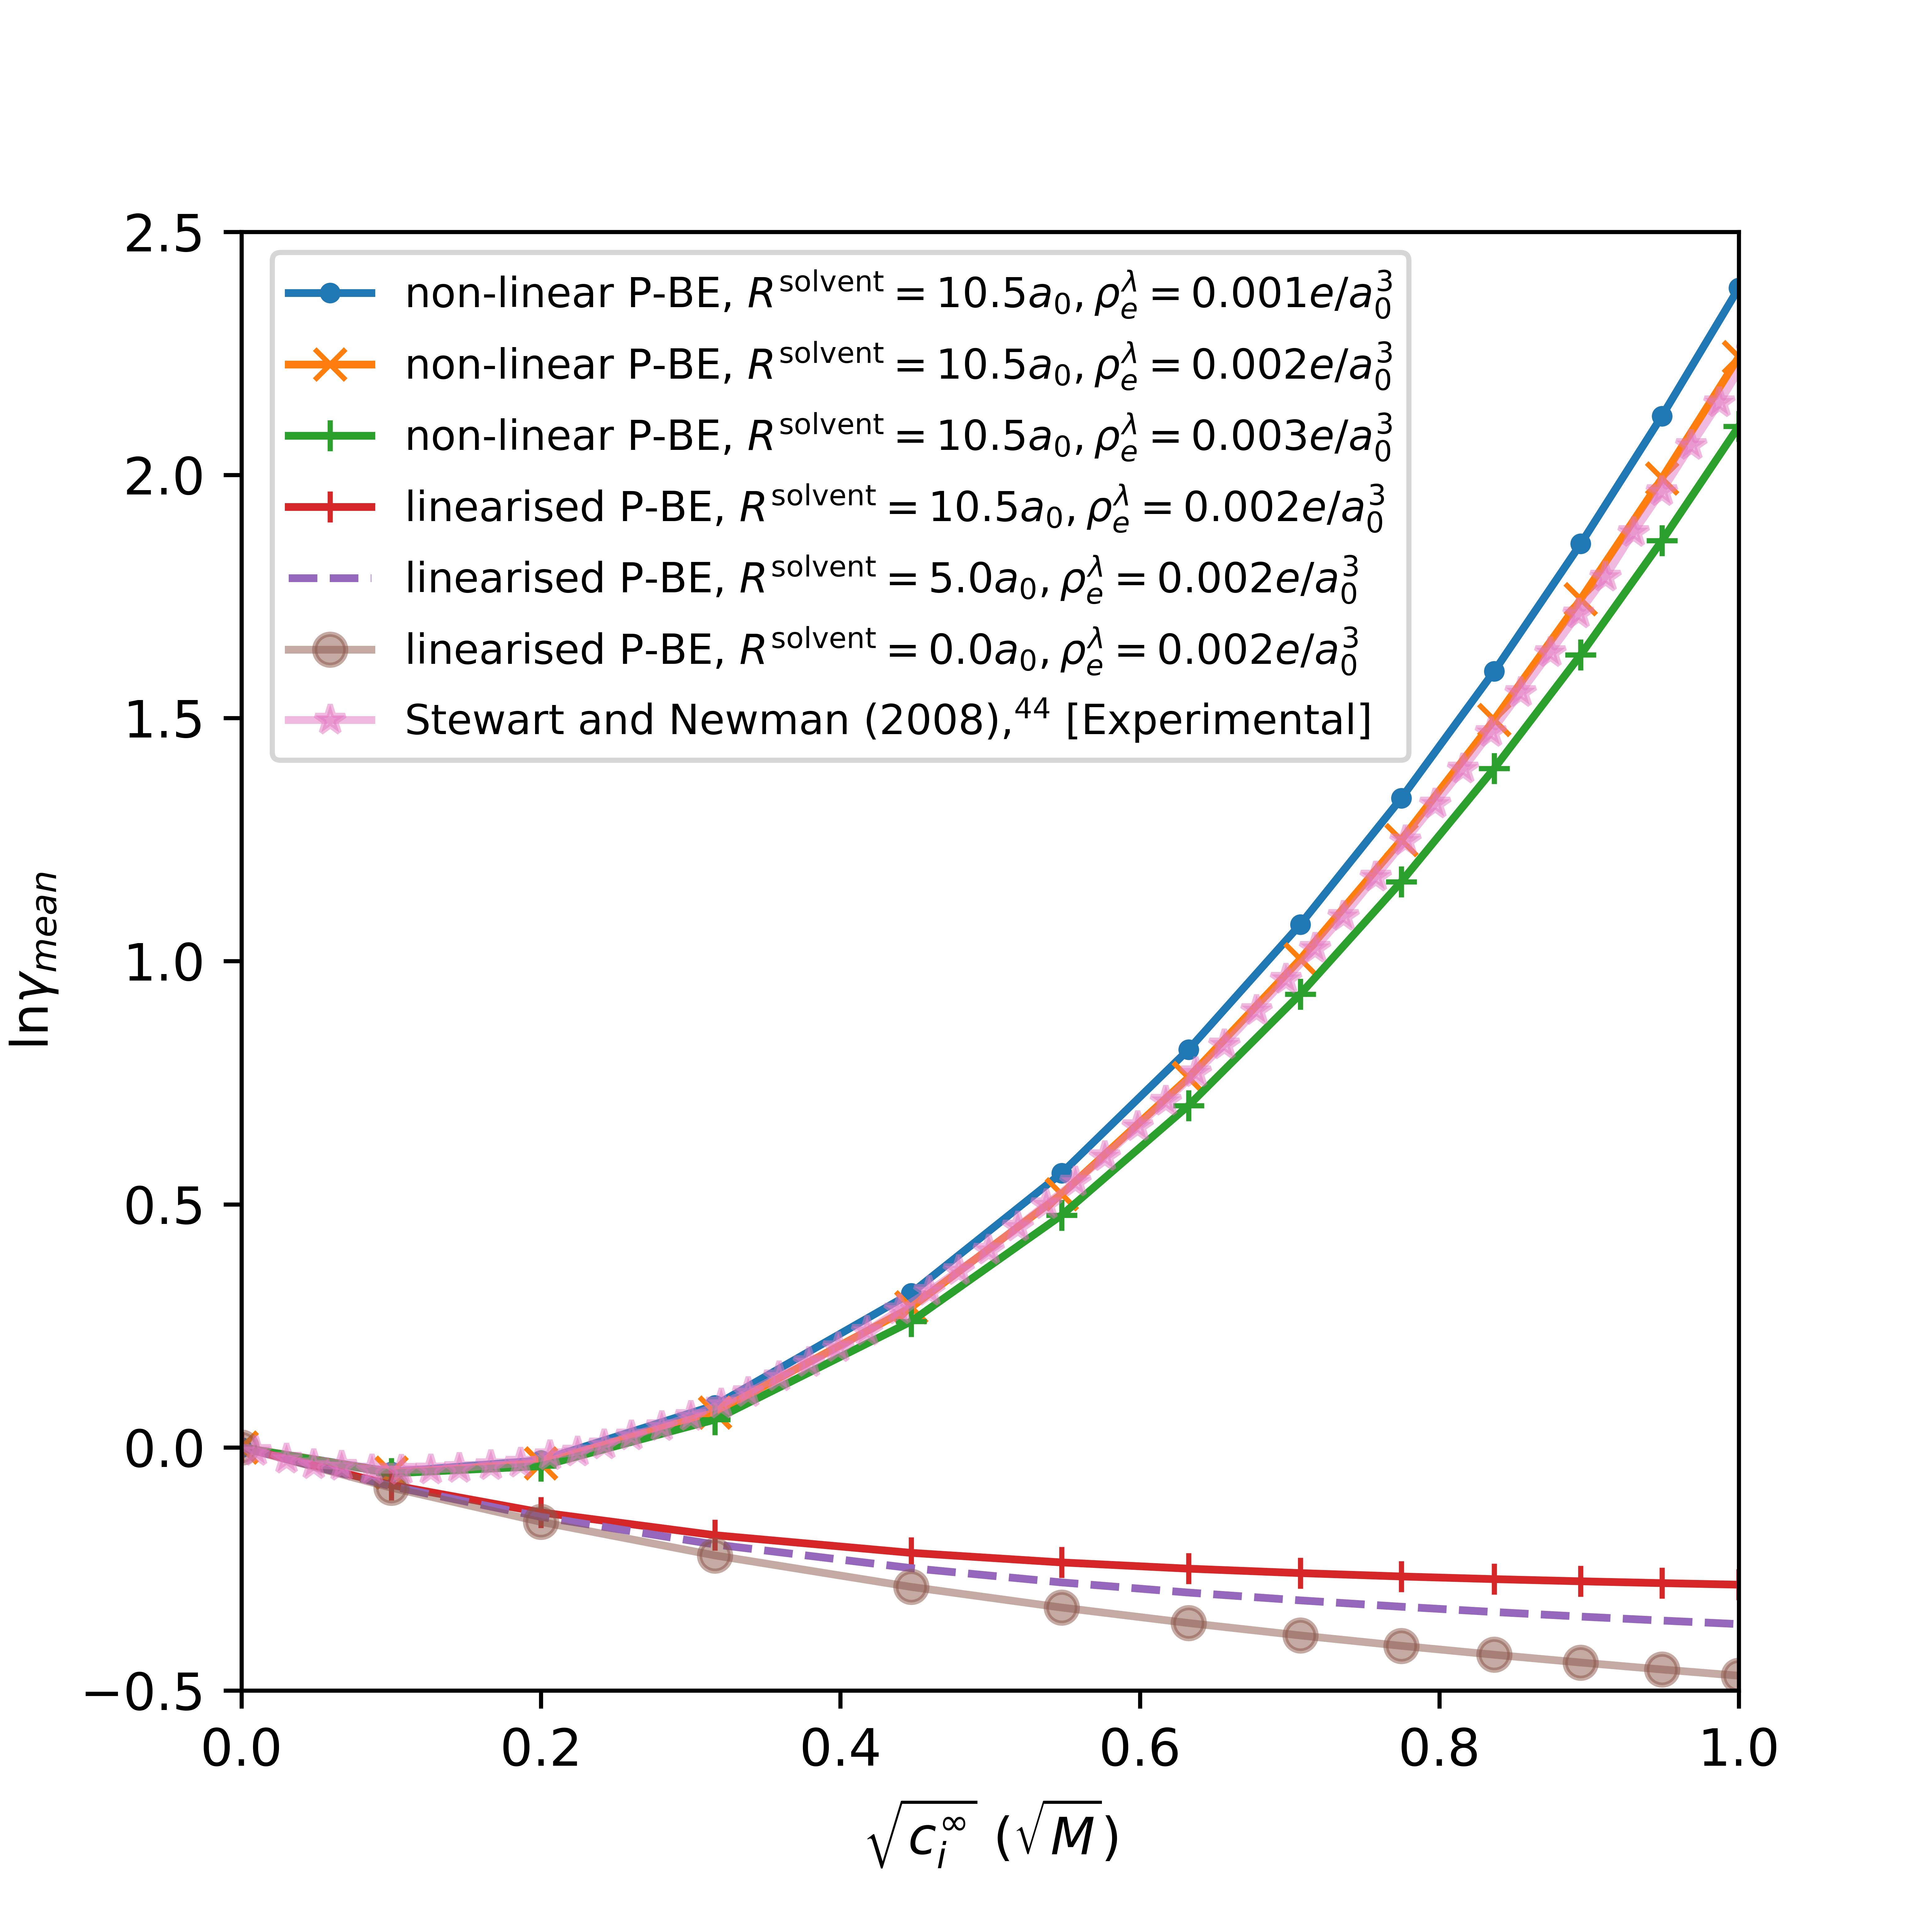
\includegraphics[scale=1]{figures/lipf6.png}
    \caption{Mean activity coefficients for LiPF$_6$ in ethylene carbonate at $T=308$~K as a function of concentration and for different values of the atomic electronic density isovalue parameter which determines the extent of the accessibility function. Calculations with the linearised approximation to P-BE are also shown. Reproduced from Ref. \citenum{Dziedzic2020}}
    \label{fig:ac}
\end{figure}
    
\subsubsection{Outlook and challenges (Arihant/Maxim)}
\begin{itemize}
    \item challenges - interatomic potentials for classical MD
    \item discrepancy between atomistic/continuum definition of "diffusion coefficient" in terms of parameterising for continuum modelling.
    \item limitation of liquid electrolytes
\end{itemize}
%end: unchanged in 30 January 2021 update

\subsection{Solid Electrolytes (Lucy/Julian/Arihant/Rana)}

\subsubsection{Introduction (Rana/Lucy/Arihant)}
%Brief History of solid electrolytes, types of solid electrolytes, types of properties which are important for batteries. Then which we will focus on in this section sulfides (using LGPS and argyrodites), oxides (Examples), composites (example).
% Possibly we can select some of the below to mention. I think the Van de Ven review covers them all, but we can focus on a few.
% Oxides - NASICONs, LISICONS, perovskites (LLTO), Li garnets, nanocomposites (ranas)
% sulfides - glass ceramics, thio-LISICON (LGPS), argyrodites.
% Others - nitrides, oxynitrides (LiPON), antiperovskites

Solid electrolytes (SE) have attracted considerable attention as an alternative to liquid electrolytes, significantly increasing the energy and power densities, improving device safety, and reducing the cost of synthesis of the battery materials. \cite{janek_solid_2016, culver_designing_2018, famprikis_fundamentals_2019, goodenough_li-ion_2013, DIRICAN201927} 
An ideal solid electrolyte material should possess  high electronic resistance, high ionic conductivity, outstanding thermal stability, strong electrochemical stability, excellent mechanical strength, and reduced interfacial resistance. \cite{han2020recent, manthiram2017} There are three different categories of solid electrolytes which are used in rechargeable batteries \cite{DIRICAN201927}: (1) Inorganic solid ceramic electrolytes, (2) Organic solid polymer electrolytes, and (3) Solid composite electrolytes. 

Solid electrolytes were discovered by Michael Faraday in the early 1830s through research on the conduction properties of heated solid sliver sulfide (Ag$_{2}$S) and lead fluoride (PbF$_{2}$) \cite{Faraday1833}. 
The use of a ceramic-based $\beta$-alumina (Na$_{2}$O$\cdot$11Al$_{2}$O$_{3}$) in high-temperature sodium-sulfur batteries in 1960s, however, was considered as a milestone in the development of batteries enabled by solid electrolytes \cite{armand2008building}. In the 1980s the Zeolite Battery Research Africa (ZEBRA) group developed the ``ZEBRA'' batteries using Na$_{2}$O$\cdot$11Al$_{2}$O$_{3}$ as the solid electrolyte. \cite{ZEBRA}
So far, the high-temperature sodium–sulfur battery has been commercialised in Japan \cite{oshima2004}, whereas the ZEBRA battery is currently being developed by the General Electric Corporation in the United States. \cite{capasso2014} 

In 1990, the Oak Ridge National Laboratory synthesised a lithium phosphorus oxynitride (LiPON) material \cite{dudney1992,bates1992}, which opened up the use of inorganic solid-state electrolytes in lithium-ion battery research. Since then, a huge number of inorganic lithium-ion conductive ceramic materials have been developed, including perovskite-type \cite{inaguma1993}, garnet-type oxides \cite{kasper1969,mazza1988}, garnet-type sulfides \cite{kennedy1986}, lithium super ionic conductor (LISICON) \cite{ivanov1988}, sodium super ionic conductor (NASICON)-like materials \cite{lang2015} and lithium-argyrodite materials. \cite{de2016}

Despite recent advancement in research activities on crystalline inorganic electrolytes, they are still brittle and therefore difficult to fit into different battery shapes. Solid-state polymer electrolytes (SPEs), due to their high flexibility, can fit in any battery shape and present improved safety and stability features compared to crystalline inorganic electrolytes. \cite{DIRICAN201927} Since 1980, various high-molecular weight dielectric polymer hosts were investigated as polymer electrolytes with high conductivities for lithium batteries, such as poly(ethylene oxide) (PEO) \cite{fenton1973}, polyacrylonitrile (PAN) \cite{abraham1990,dautzenberg1994}, poly(vinylidene fluoride) (PVDF) \cite{arcella1999,kataoka2000,li2016}, poly(methyl methacrylate) (PMMA) \cite{appetecchi1995,bohnke1993} and poly(vinylidene fluoride-hexa-fluoropropylene) (PVDF-HFP) \cite{abbrent2001,park2008,yang2014}.

The ionic conductivities of most polymer electrolytes are significantly lower than those of both oxide solid electrolytes and liquid electrolytes. \cite{zhou2016} A possible solution to this limitation is to create composites by integrating nanoscale highly-conductive inorganic particulate fillers into the polymer electrolyte material. \cite{DIRICAN201927} This enhances the ionic conductivity and also improves the mechanical strength and stability of the solid-state polymer electrolytes, including the interfacial stability. \cite{D0SC03121F} Here, heterogeneous doping increases the ionic conductivity as a result of increasing interfacial regions between an inert solid phase, such as silica or alumina or boron oxide particles and an electrolyte. \cite{uvarov2011} A wide range of inorganic solid composite electrolytes have previously been studied, based on oxides (Li$_{2}$O:Al$_{2}$O$_{3}$ \cite{B300908D}, Li$_{2}$O:B$_{2}$O$_{3}$ \cite{Heitjans_2003,Indris2000,Indris2002}), hydrides (LiBH$_{4}$:SiO$_{2}$ \cite{blanchard2015}), halides (LiI:Al$_{2}$O$_{3}$ \cite{liang1973}, LiI:SiO$_{2}$ \cite{phipps1983}, LiF:Al$_{2}$O$_{3}$ \cite{uvarov1992}), and sulfides (Li$_{2}$S:SiS$_{2}$ \cite{pradel1986}). 

The high ion conductivities of liquid electrolytes have, thus far, been unreachable for solid electrolytes, however, research efforts over the last decade have presented a limited number of promising candidates with high ionic conductivities ($>$1 mS cm$^{-1}$) as a potential competitive to liquid electrolytes.\cite{kanno_synthesis_2000,murayama_synthesis_2002,murayama_material_2004,minafra_influence_2019,bron_li_2013,whiteley_empowering_2014,huang_superionic_2019,yamane_crystal_2007,homma_crystal_2011} Figure \ref{fig:solid-electrolyte} presents a plot by \citeauthor{Kamaya2011} with the ionic conductivities of most currently known solid electrolytes.

\begin{figure}[htbp]
    \centering
    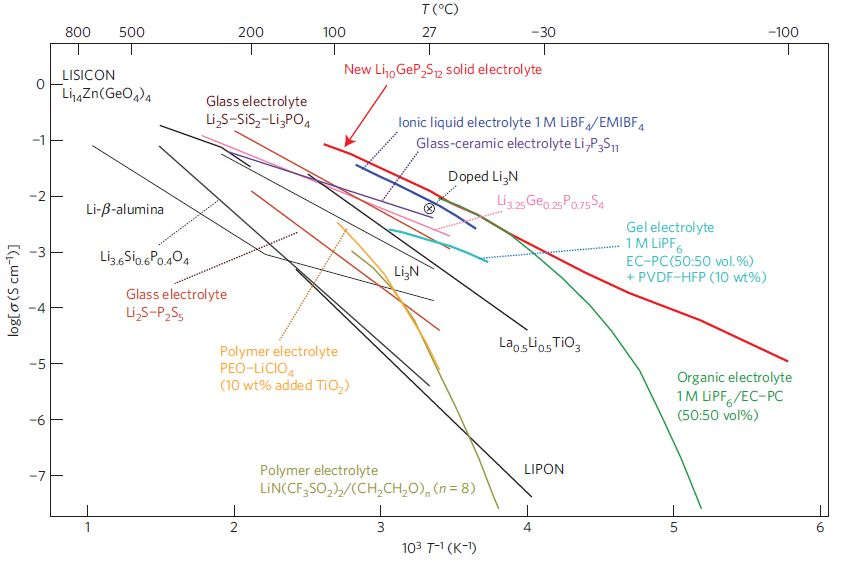
\includegraphics[scale=0.6]{figures/kamaya.jpg}
    \caption{Ionic conductivity of different solid electrolytes, reproduced with permissions from Ref. \citenum{Kamaya2011}}
    \label{fig:solid-electrolyte}
\end{figure}

In this section, we review atomistic modelling investigations into the structure-property relationships in selected solid-state electrolytes; Li$_{10}$GeP$_2$S$_{12}$ (LGPS), lithium argyrodites, and Li$_7$La$_3$Zr$_2$O$_{12}$ (LLZO) which belong to the inorganic solid ceramic electrolyte type and Li$_{2}$O:B$_{2}$O$_{3}$ materials which belong to the oxide based solid composite type. A particular focus is given on the ion transport mechanism in those materials which is important for reaching high conductivities, a key property of battery materials. Finally, we take a more detailed look at the interface of solid electrolytes with the electrodes, and discuss the challenges and outlook for future atomistic modelling investigations.

\subsubsection{Sulfides (Arihant/Lucy)}
There are a larger number of computational studies of sulfides which partly related to a recent increase in newly discovered crystalline sulfide superionic conductors. Sulfides also tend to have comparatively lower intrinsic electrochemical and chemical stability, which has stimulated interest for understanding the interfacial interactions within batteries. \cite{Xiao2020interfacerev} The sulfide group encompasses a range of sulfide based solid electrolytes, including, glass ceramics \cite{minami2006recent}, argyrodites \cite{bai2020research}, and thio-LISICONs \cite{minafra2020two}. Some of the most promising SEs to emerge in recent years include the Li$_{10}$GeP$_2$S$_{12}$ (LGPS) \cite{Bhandari2016,Kamaya2011,Mo2012} and the Li-argyrodite (Li$_6$PS$_{5}X$, $X$=Cl,Br,I) \cite{kraft2018,deiseroth_li6ps5x_2008,deklerk2016,kraft2017,minafra2018,adeli2019} families of superionic conductors.

\textbf{LGPS}
The crystal structure and the phenomenal conductivity of Li$_{10}$GeP$_2$S$_{12}$ was reported by \citeauthor{Kamaya2011}, presenting the highest room temperature ionic conductivity (12 mS/cm) among all other solid electrolytes, Fig.~\ref{fig:solid-electrolyte}. \cite{Kamaya2011} \citeauthor{Kamaya2011} determined that diffusion in LGPS is anisotropic where the $c$ directional motion dominates over the $ab$ plane, with an overall energy barrier for Li diffusion being 0.24 eV. The discovery was followed by an ab-initio MD study by \citeauthor{Mo2012}, who determined an average energy barrier of 0.17 eV along the $c$ channel and 0.28 eV in cross channel direction, i.e. along the $ab$ plane.\cite{Mo2012} Further to this, \citeauthor{Xu2012one} found that the Li atoms move along the $c$ channels in a cooperative way, instead of through the nearest neighbor hops, due to the large coulombic repulsion between them.\cite{Xu2012one} \citeauthor{Adams2012} performed a molecular dynamics study and predicted the presence of additional Li sites which would provide diffusion along the $ab$ plane.\cite{Adams2012} The additional sites could change the diffusion scenario altogether, by not only changing the occupancies of Li in the $c$ channel, but also by providing a diffusion mechanism involving $ab$ plane. \citeauthor{Kuhn2013a} confirmed the presence of these additional sites experimentally by performing single crystal XRD.\cite{Kuhn2013a} The interesting discovery of additional sites has opened up the possibility of cross-channel mechanisms of ion movement. \citeauthor{Kuhn2013b}, in a further study, reported that the diffusion in LGPS is more or less isotropic with an overall activation energy barrier of 0.22 eV.\cite{Kuhn2013b}

\citeauthor{Bhandari2016} performed a first-principles DFT study of Li diffusion energy barrier via the nudged elastic band (NEB) method, taking into account the fractional occupancies leading to variable $c$ channel Li populations, variable chemical environments surrounding Li, and all possible migration mechanisms.\cite{Bhandari2016}  They found that the Li diffusion is neither purely $c$ directional nor purely along the $ab$ plane, but there exists a correlated mechanism of motion along $c-ab$ which critically controls the degree of anisotropy of Li diffusion in LGPS. The energy barriers for different mechanisms of Li-diffusion are shown in Fig. \ref{fig:lgps}, which suggests that the correlated hop has the lowest energy barrier. This correlated mechanism of Li-diffusion could not be deciphered from the experimental data or MD data alone, as these methods can only isolate diffusivities along particular directions. \citeauthor{Bhandari2016} further performed a statistical average of all diffusion energy barriers, taking into account the formation energy of various Li configurations and predicted an overall energy barrier of 239 meV, which is in close agreement with experiments.\cite{Kamaya2011} Thus, the first-principles approach not only explained the overall diffusivities and energy barriers, but also gave insight into the underlying mechanism behind the fast Li diffusion in LGPS and resolved the discrepancy about the anisotropy of Li diffusion in this compound.

\begin{figure}
    \centering
    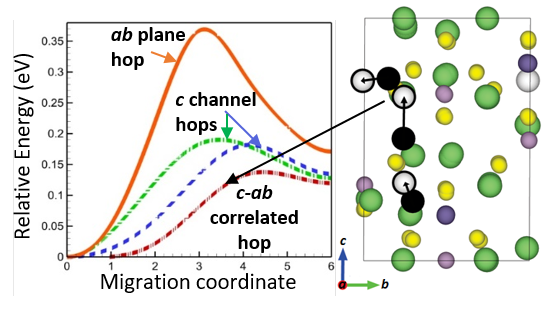
\includegraphics[scale=1.2]{figures/lgps.png}
    \caption{Energy barrier for Li-ion diffusion in LGPS solid electrolyte calculated using NEB method. Reproduced from Ref. \citenum{Bhandari2016}}
    \label{fig:lgps}
\end{figure}

\textbf{Lithium argyodites}, Li$_6$PS$_{5}X$ ($X$= Cl,Br,I) can reportedly reach ionic conductivities of up to $10^{-2}$. \cite{deiseroth_li6ps5x_2008} While Li$_6$PS$_{5}$Cl and Li$_6$PS$_{5}$Br exhibit high ionic conductivities of $10^{-3}$ Scm$^{-1}$ at room temperature, Li$_6$PS$_{5}$I has considerably lower conductivitives of $10^{-6}$ Scm$^{-1}$.The three orders of magnitude difference is surprising as the identical crystal structures suggest the same Li diffusion pathways exist in all systems. Another intriguing aspect is that the conductivity trend runs counter to other families of SEs, such as LGPS, where larger, more polarisable and less electronegative anions are linked with increased ionic conductivites. \cite{bachman2016inorganic}

Understanding which properties and mechanisms influence the conductivity is essential to obtaining higher ionic conductivities and improving battery performance. Material stoichiometry, anion/cation disorder, and doping, have all been shown to influence conductivities. The effect of these can be difficult to deconvolve in many materials as they are intrinsically coupled in experimental systems. This is where computational analysis can provide vital insight, allowing deconvolution of coupled properties and the roles they play in the diffusion process.

A particularly interesting aspect of the Li-argyrodites is the diffusion topology, which comprises of interconnected Li$_6$S cages, with anions arranged at 4a, 4c, and 16e Wyckoff positions and Li arranged over type 1, 2, 4, and 5 tetrahedra.\cite{kuhs1979} Lithium mainly occupies type 5 tetrahedral sites in $x$(Li)=6 argyrodites, with occupation of non-type 5 sites only recently observed experimentally. \cite{ohno2019further,gautamengineering} Computational studies however have previously predicted occupation of non-type 5 sites, showing lithium distributed over tetrahedral types 5, 2, and 4. \cite{deiseroth_li6ps5x_2008, Minafra2020, morgan2020mechanistic}

Li hopping within these cages, while effectively barrier-less, does not contribute to long-range diffusion. In fact, a combination of inter-cage and intra-cage hopping is needed, with occupation of non-type 5 sites and transitions between all adjacent site types to achieve long-range diffusion. This is shown schematically in Figure~\ref{fig:diffusion_pathways} showing the connectivity between the Li tetrahedral sites. AIMD simulations have shown that cation and anion substitution \cite{ohno2019further,deklerk2016}, anion site disorder \cite{gautamengineering,morgan2020mechanistic}, and lithium concentration \cite{Deng2017, yu_superionic_2020, Feng_2020}, all influence the ionic conductivity.

\begin{figure}
    \centering
    
\includegraphics[scale=0.65]{figures/diffusion_pathways.pdf}
    \caption{(a) Possible Li diffusion pathways in Li-argyrodites involving types 2, 4, and 5 tetrahedra for long range diffusion. Ref. \citenum{morgan2020mechanistic}}
    \label{fig:diffusion_pathways}
\end{figure}

The influence of anion substituent concentration on conductivity is currently uncertain, with research by \citeauthor{deklerk2016} determining excess Cl in Li$_5$PS$_4$Cl$_2$ resulting in similar conductivities to Li$_6$PS$_5$Cl \cite{deklerk2016}, in contrast to research by \citeauthor{yu2019tailoring} and \citeauthor{Feng_2020} concluding excess Cl improved Li conductivity. \citeauthor{yu2019tailoring} determined the highest conductivity was produced by Li$_{5.7}$PS$_{4.7}$Cl$_{1.3}$ (6.4 mS cm$^{-1}$), \cite{yu2019tailoring,yu_superionic_2020} while \citeauthor{Feng_2020} determined this to be Li$_{5.3}$PS$_{4.3}$Cl$_{1.7}$ (17 mS cm$^{-1}$). \cite{Feng_2020} \citeauthor{Feng_2020}, however, presented alternative, or coupled, reasoning for this increased conductivity. Drawing from previous studies \cite{adeli2019,zhou_solvent-engineered_2019} they propose the increased Cl content amplified the anion disorder in the system, which is the underpinning cause of the higher conductivities.

\subsubsection{Oxides (Julian/Rana)}
\label{sec:se_oxides}

% \begin{itemize}
%     \item Intro
%     \item LLZO (Julian)
%     \item Nanocomposites (Rana)
% \end{itemize}

\textbf{LLZO} Cubic Li$_7$La$_3$Zr$_2$O$_{12}$ (c-LLZO) shows its promise as a solid electrolyte by fulfilling a number of criteria essential for this role. It has a high Li-ion conductivity (\(3\times 10^{-4}\,\mathrm{Scm}^{-1}\))\cite{Murugan2007}, a high shear modulus (59\,GPa)\cite{Ni2012}, and the largest thermodynamic stability window against lithium metal\cite{Zhu2016, Binninger2020} of current solid electrolyte materials. However, c-LLZO is not a stable phase at room temperature.\cite{Geiger2011} At lower temperatures (\(<150 ^\circ C\)) a phase transition occurs forming the much less ionically conductive tetragonal LLZO (t-LLZO) phase.\cite{Geiger2011} In order to retain the more ionically conductive cubic phase at lower temperatures, Al doping on lithium sites was found to be a good solution.\cite{Geiger2011, Rangasamy2012}

Despite the appealing characteristics of this material, lithium dendrite growth has proven to be a problem that has caused short circuits in LLZO cells after relatively short periods of use \cite{Ren2015,Sudo2014}. This growth has been observed directly by \citeauthor{Cheng2017}, who found that this process occurs mostly through grain boundaries.\cite{Cheng2017} \citeauthor{Kim2020} corroborated this observation and investigated the use of an interlayer buffer as a means to restrict Li propagation through grain boundaries.\cite{Kim2020}

\citeauthor{Monroe2004} predicted, through the classical kinetic modelling of an electrode-solid electrolyte interface, increasing surface stability with increasing shear modulus for solid electrolytes.\cite{Monroe2004, Monroe2005} It is therefore surprising that dendrite growth occurs in LLZO which has respectively large shear modulus compared to other solid electrolytes. However, the authors do note that their models do not account for fracturing of a brittle material.

The potential of this material coupled with its apparent dendrite issue has led to a number of attempts to model this formation computationally\cite{Canepa2018, Tian2018, Gao2020}. \citeauthor{Tian2018} provided rigorous computational evidence for the mechanism by which these dendrites form using DFT (described in sec. \ref{sec:dft}). \cite{Tian2018} Firstly, the total density of states (TDOS) of the lowest energy surface slab and bulk structures were compared for c-LLZO and t-LLZO. t-LLZO forms at the surface of bulk c-LLZO even with Al-doping\cite{Ma2016, Rettenwander2018}. This comparison revealed that there were extra states in the band gap for slab structures and thus a possibility for electrons to be trapped on the surface of LLZO. Next, the localisation of the electrons on the surface was found by adding extra electrons to the structures and comparing the charge density to that of the original. It was found that localisation occurred primarily around Li$^+$ and La$^{3+}$ ions on the surface. Finally, the authors wanted to ensure that it was thermodynamically favourable to reduce the Li$^+$ over the La$^{3+}$ ions by analysing the thermodynamic driving force for the products of Li$_2$O and La$_2$O$_3$. The lithium product was found to be more favourable and so they concluded that the trapping of electrons on the surface led to the nucleation of lithium metal. This could lead to growth through grain boundaries and pores in the LLZO eventually forming dendrites\cite{Ren2015}, Fig. \ref{fig:tian2020}. The authors also looked at Li$_2$PO$_2$N (LiPON) through the same tests and found no electron trapping occurs. This indicated it may make a suitable coating to prevent dendrite and t-LLZO formation.

\begin{figure}[H]
    \centering
    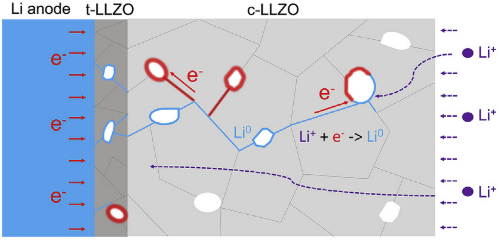
\includegraphics{figures/tian_grain_growth.png}
    \caption{Schematic showing Li metal formation (blue) along grain boundaries and pores due to electron accumulation (red) combining with Li$^+$ as they move through the electrolyte. From Ref. \citenum{Tian2018}}
    \label{fig:tian2020}
\end{figure}

This theory for the dendrite growth mechanism is contradicted by \citeauthor{Gao2020} who attributed it to the under-coordination of Zr present on some of the more stable surfaces of LLZO .\cite{Gao2020} This under-coordination may lead to inhomogenous Li depletion which can lead to Li metal depostion and dendrite formation.\cite{Tsai2016} The apparent rift between these two papers stems from the choice of surface. \citeauthor{Tian2018} argue that lithium and lanthanum rich surfaces are more stable based upon the the research conducted by \citeauthor{Thompson2017}, where DFT calculations on 6 different LLZO slabs for the 100 and 110 planes, was performed. In contrast, \citeauthor{Gao2020} drew upon results presented in several methods\cite{Thompson2017, Canepa2018, Yu2016a} and performed DFT calculations on a wider range of surfaces, finding 100 and 001 surfaces the most stable. They also agreed with the findings of \citeauthor{Tian2018} with respect to Li and La rich surfaces being the most stable. \citeauthor{Gao2020} however, went a step further and analysed the Li-LLZO interface using the CALYPSO interface structure prediction method\cite{Wang2012, Gao2019}, which calculated the interface formation energies. They found the Zr-rich surfaces tended to form the most stable interfaces with the Li anode. Zr being the cause of interfacial instability has been confirmed with the experimental findings of \citeauthor{Zhu2019} \cite{Zhu2019}.

Some experimental papers have suggested that one of the primary causes of dendrite growth is a reduction of Li ions in bulk LLZO due to a non-uniform distribution of current on the surface.\cite{Han2019_dendrite, Aguesse2017}
A preprint by \citeauthor{squires_2020} sought to model electronic conductivity in LLZO in order to probe how large a part this property played in dendrite formation.\cite{squires_2020} DFT calculations were used and the results fed in to a novel workflow to find the electronic conductivity from first principles. The authors found that at room temperature, bulk c-LLZO had negligible electron/electron-hole concentrations indicating that bulk defects are not a significant factor in dendrite growth. However, the authors do mention that their model does has not been applied to other forms of defects such as grain boundary and surface effects which could be a causes of the non-uniform distribution of current reported. 

\citeauthor{Xu2012} analysed the Li-ion migration path through LLZO using DFT and found two migration paths were possible, depending on Li concentration.\cite{Xu2012} Low Li concentration (around Li$_5$La$_3$Zr$_2$O$_{12}$) led to a higher energy, single hop, migration path. At higher Li concentrations (around Li$_7$La$_3$Zr$_2$O$_{12}$), however, this route became more complex and led to a lower energy, two hop, migration path. This was found using the nudged elastic band (NEB) method (see sec. \ref{sec:methods_neb}).

\citeauthor{Burbano2016} used classical molecular dynamics (see sec. \ref{sec:molecular_dynamics}) to find a more robust description of the ion transport mechanism.\cite{Burbano2016} The interatomic potentials were found using a hybrid DFT functional. The authors put an emphasis on the difference in ionic conductivity between t-LLZO and c-LLZO. They found the longer time scale of classical MD allowed the observation of a large sample of diffusion events in both LLZO structural forms (see fig. \ref{fig:burbano_diffusion}). It was found that diffusion events in t-LLZO were far less common and that most of those diffusion events involved exactly 8 Li ions. The significance of precisely 8 Li ions being involved in these events is that it relates to the cyclic movement of Li ions about a ring of 12 octahedral an tetrahedral sites in t-LLZO. This diffusion mechanism results in no net diffusion of Li and hampers the ability of t-LLZO to conduct ions. 

\begin{figure}[h]
    \centering
    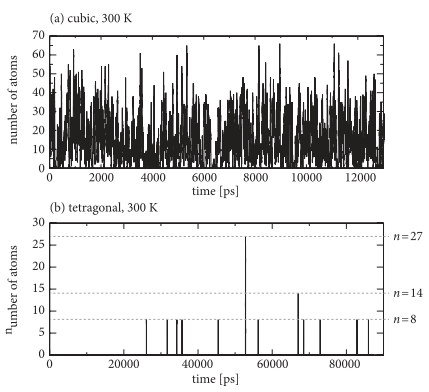
\includegraphics[scale=1]{figures/burbano_diffusion_events.png}
    \caption{Excitation states or diffusion events at 300 K for c-LLZO (a) and t-LLZO (b). Each line represents a diffusion event that affects a number of lithium ions. t-LLZO has far fewer of these events making it necessary to sample it at a much longer timescale. }
    \label{fig:burbano_diffusion}
\end{figure}

Previous papers on the issue have used AIMD to investigate the transport mecahnism in LLZO
%(see sec. \ref{sec:aimd}.
AIMD samples at a much smaller time scale. This led to some key disagreements about the transport mechanism in c-LLZO.\cite{Meier2014, Jalem2013, Burbano2016}

More recently \citeauthor{Bonilla2019} applied classical MD to investigate the ionic conductivity in Al-doped LLZO.\cite{Bonilla2019} DFT calculations had previously revealed that Al doping reduces the energy barrier for Li-ions to move between octahedral and tetrahedral sites.\cite{Rettenwander2014, Rettenwander2016} this was supported by the findings of \citeauthor{Bonilla2019} who went on to conclude that there is an increase in conductivity in t-LLZO due to the Al forcing Li ions into previously inaccessible tetrahedral sites. However, the authors also found a slight decrease in conductivity as Al was doped in c-LLZO. They attributed this to the tendency for Al to "trap" Li ions close to the dopant.

A recent, comprehensive review of experimental and computational techniques used in order to probe ion transport mechanisms can be found in ref. \citenum{Gao2020_ion_transport}.

\citeauthor{Sharafi2017} investigated the apparent low wettability of Li  on LLZO using DFT.\cite{Sharafi2017} The authors found the adhesive energy using:

\begin{gather}\label{eq:adhesive_energy}
    W_{ad}=E_{int}-E_{Li-slab}-E_{LLZO-slab}
\end{gather}

where $E_{int}$ is the interface energy and $E_{X-slab}$ the energy of the individual slabs. The adhesive energy can then be used to calculate the wetting angle by using the Young-Dupr\'e equation:

\begin{gather}\label{eq:young_dupre}
     W_{ad}=\sigma_{Li}(1+\cos{\theta})
\end{gather}

where $\sigma_{Li}$ is the surface energy of Li and $\theta$ is the contact angle. \citeauthor{Sharafi2017} found the calculations to be in good agreement with the experiments conducted within the paper.

Atomistic modelling has proven useful in probing the properties of LLZO. It has revealed insights in dendrite growth, ion transport, thermodynamic stability, electronic conductivity and Wettability. Atomistic modelling has moved away from the bulk material and is looking at the interfaces formed with LLZO and other solid electrolytes (see sec. \ref{sec:interface_stability}) as well as investigating the effectiveness of various coatings in mitigating some of the unfavourable properties outlined in this section. 

\textbf{Oxide Nanocomposites} Due to attractive mechanical, electrical, optical, and magnetic properties nanocomposite oxide materials represent a new generation of advanced materials. \cite{uvarov2011,Heitjans_2003} They often show enhanced conductivity compared to the single-phase ceramic oxides which makes them suitable candidates as electrolytes for future solid state batteries. For example, Li$_2$O:B$_2$O$_3$ \cite{Heitjans_2003,Indris2000,Indris2002} and Li$_2$O:Al$_2$O$_3$ nanocomposites \cite{B300908D} have higher ionic conductivities than nanocrystalline Li$_2$O, although B$_2$O$_3$ and Al$_2$O$_3$ are insulators. The ionic conductivity shows a maximum at about 50 \% of B$_2$O$_3$/Al$_2$O$_3$ content. This surprising behaviour was attributed to the increased fraction of structurally disordered interfacial regions and the enhanced surface area of the nanosized particles \cite{Heitjans_2003}. The oxide nanocomposites contain three types of interfaces, as presented in Fig.~\ref{fig:LBO} (a): interfaces between the ionic conductor grains (green lines), between the insulator grains (black lines), and between the ionic conductor and the insulator grains (red lines). The latter can lead to surprising effects in the conductivity of composite materials. In this case, the highly conducting interface region can act as a bridge between two Li$_2$O grains not in direct contact with each other, opening up additional paths for Li ions. The conductivity enhancement in the interfacial regions may have different origins, e.g. the formation of space charge layers, an enhanced concentration of dislocations, or defects or the formation of new phases.

\begin{figure}
    \centering
    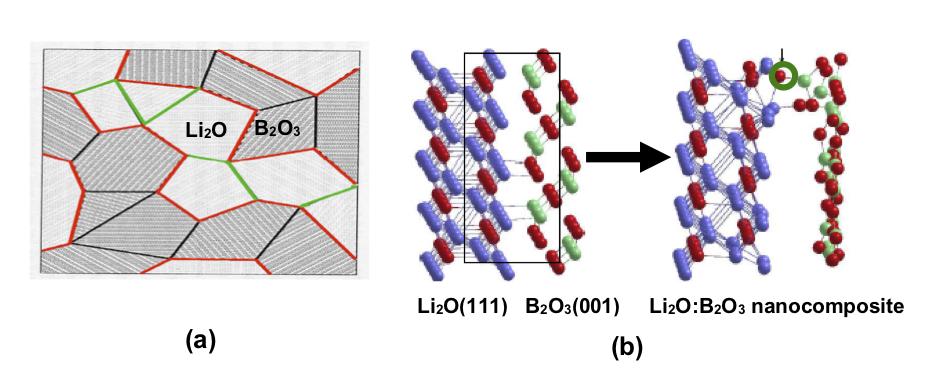
\includegraphics[scale=1]{figures/Islam-Fig-Li2O-B2O3.png}
    \caption{(a) Schematic diagram of Li$_2$O and B$_2$O$_3$ interface (Reproduced from ref. \citenum{Heitjans_2003}). (b) Atomistic model of Li$_2$O:B$_2$O$_3$ nanocomposite ref. \citenum{Rana-JPCM-2012}.}
    \label{fig:LBO}
\end{figure}

\citeauthor{Rana-PRL-2007} studied the interface of Li$_2$O:B$_2$O$_3$ nanocomposite by modelling a combination of two favorable surfaces of Li$_2$O and B$_2$O$_3$ using HF/DFT Hybrid approach. \cite{Rana-PRL-2007,Rana-JPCM-2012} After full structural optimisation, it was observed that Li--O bonds are weakened and simultaneously B--O bonds are formed at the boundary between the two surfaces, Fig. \ref{fig:LBO} (b). An oxygen atom from the Li$_2$O surface (marked by a green circle) is pulled from the surface layer towards a neighboring boron atom of the B$_2$O$_3$ surface. This preference of oxygen bonding with B (or Al in Li$_2$O:Al$_2$O$_3$) plays a key role in generating low-coordinated Li. As a consequence of this dislocation, the coordination of a Li atom in the second layer is reduced from four to three. 

The defect properties were investigated in the interface region. It was observed that the removal of surface oxygen from Li$_2$O is responsible for the increased vacancy defect concentration in Li$_2$O:B$_2$O$_3$ (or Li$_2$O:Al$_2$O$_3$) nanocomposite materials. Therefore the nanocomposites of ionic compounds (containing weakly bound and therefore mobile cations) with highly covalent compounds (with strong metal- or nonmetal-oxygen bonds) are in general promising candidates for high ionic conductivity. The model calculations showed that the most likely mechanism for Li$^+$ migration was in a zigzag pathway rather than in a straight line along a direction parallel to the interface plane. 

The average calculated activation energy for Li$^+$ migration in the Li$_2$O:B$_2$O$_3$ interface (0.28 eV) \cite{Rana-PRL-2007,Rana-JPCM-2012} is similar to the experimental values of bulk Li$_2$O (0.31 eV) \cite{Heitjans_2003}, Li$_2$O:B$_2$O$_3$ ($0.34 \pm 0.04$ eV) \cite {Indris2002} and Li$_2$O:Al$_2$O$_3$ ($0.30 \pm 0.02$ eV) \cite{B300908D} nanocomposites. According to the defect formation energies, the interface region of Li$_2$O:B$_2$O$_3$ nanocomposites contains higher concentrations of both Li vacancies and Frenkel defects than bulk Li$_2$O and the Li$_2$O surfaces. \cite{Rana-PRL-2007,Rana-JPCM-2012} Therefore the experimentally observed enhanced Li mobility in the Li$_2$O:B$_2$O$_3$ interface region is thermodynamically and not kinetically controlled. Models as proposed in that study allowed a direct simulation of the defect formation and ion mobility at atomic scale without any experimental input. They provided a deep insight into the local bonding situation at the interface of oxide nanocomposites which was difficult to obtain from experiments.


\subsubsection{Interface stability (Julian)}
\label{sec:interface_stability}

Atomistic modelling has proven to be a useful asset when examining solid electrolyte interfaces as probing the interfaces experimentally is often difficult\cite{Xu2018exp}.An in-depth experimental and computations review on solid electrolyte interfaces is given by \citeauthor{Xiao2020interfacerev} \cite{Xiao2020interfacerev} Here, we focus on an overview of the atomistic modelling contributions to the investigation of these interfaces. 

It was widely reported in both experiment\cite{Liu2013, Han2015} and theory\cite{Mo2012} that certain solid electrolytes have an electrochemical stability window against a Li anode between 0--5 V.\cite{Kamaya2011, Thangadurai2005, Liu2013} \citeauthor{Mo2012} reported a 3.6 eV band gap from a DFT calculation (cf. section~\ref{sec:dft}) for LGPS.\cite{Mo2012} They attributed this to the extra stability observed in experiment to the passivisation phenomenon forming a SEI at the interface of the anode-electrolyte.\cite{Kobayashi2008}
More recent work has questioned this high stability window. \citeauthor{Zhu2015} demonstrated using DFT, that the stability windows, particularly sulfides, are far smaller than originally thought (fig.~\ref{fig:se_stab}).\cite{Zhu2015} 

\begin{figure}[H]
    \centering
    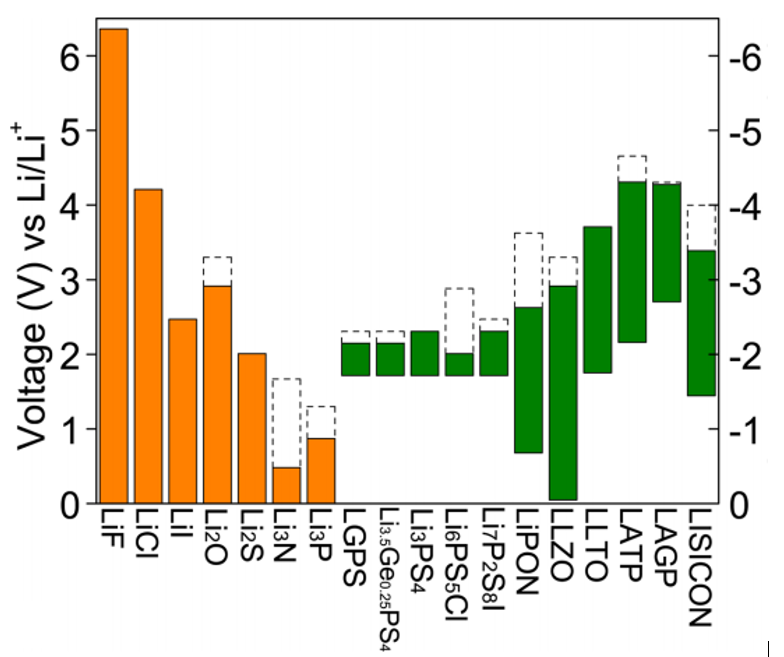
\includegraphics[scale=0.5]{figures/SE_voltage_stability.png}
    \caption{A comparison of the voltage stability windows for a selection of solid electrolytes (green) and the binary compounds that often form upon decomposition of the solid electrolyte (orange). The dashed line represents the oxidation potential to fully delithiate the material. From Ref. \citenum{Zhu2015}}
    \label{fig:se_stab}
\end{figure}

The significance of the reduced thermodynamic window is that it places a higher importance on the interphase layer formation. In general \citeauthor{Zhu2015} found these solid electrolytes to be unstable with respect to Li metal at low and high voltages with the exception of LLZO that appears to be kinetically stabilised at low voltage as it has an unfavourable reduction energy of only -0.02 eV per atom. Any potential outside of the solid electrolyte's thermodynamic stability window (fig. \ref{fig:se_stab}) results in decomposition into lithium binary compounds. This is problematic for germanium and titanium containing compounds as they form electronically conductive alloys.\cite{Zhu2015} This renders the proposed passivation process impossible\cite{Mo2012, Zhu2015} as this degradation would be sustained throughout the bulk cycling severely limiting the efficacy of these materials as electrolytes. Other solid electrolytes face different problems. As explained in sec. \ref{sec:se_oxides}, LLZO forms the far less ionically conductive tetragonal LLZO at the surface. The Li-LiPON and Li-argyordites interfaces were reported to degrade favourably, forming an ionically conductive and electronically insulative interphase consisting of Li2O, Li2S, Li3P, Li3N, and LiI.\cite{Zhu2015} 

%Investigations into a range of interfaces have been conducted. A summary of these investagations and their major findings are listed below. 
%\begin{itemize}
%    \item Li$_3$PO$4$/Li\cite{Lepley2015}
%    \item Li$_3$PO$4$/Li\cite{Lepley2015}
%    \item LLZO/Li \cite{Sharafi2017}
%    \item 
%\end{itemize}

Further study by \citeauthor{Zhu2016} sought to investigate the mechanism behind the degradation/instability at the surface.\cite{Zhu2016} In order to probe this they looked at several solid electrolytes (LGPS, LLZO, LiPON, NAISICON-type, LLTO) and calculated the chemical stability, electrochemical stability and the equilibrium conditions at the interfaces. Examining the cathode-electrolyte interface, using lithium cobalt oxide (LCO), a similar pattern emerged. Oxides were far more stable than their sulfide counterparts. However, LLTO and LATP had the best electrochemical stability against LCO. LLZO still performed well. 

Studies looking into the interfacial resistance have been conducted. \citeauthor{Tateyama2019} attributed the main source of the resistance to the electric double layer which in liquid electrolytes consists of a capacitance and diffusion layer.\cite{Tateyama2019} They investigated this by using the CALYPSO method to find low-energy surfaces\cite{Gao2019} as they could not use typical Molecular Dynamics methods, due to computational costs, to probe the interface as done with liquid electrolytes (see sec. \ref{sec:Liquid_electrolytes}). Once stable interfaces were found, the lithium chemical potential in the Helmholtz layer could be found. This corresponds to the negative of the Li ion vacancy formation energy. These energies correspond to where the the lithium will move from the electrode to the electrolyte first. These sites depleting first upon charging can be a source of interfacial resistance. 

A study by \citeauthor{Lepley2015} used DFT to investigate the interface energies between the Li electrode and the compounds that make up the interphase layer of the electrolyte.\cite{Lepley2015} They defined the interface energy as 

\begin{gather}
    \gamma_{ab}(\Omega)=\frac{E_{ab}(\Omega,A,n_a,n_b)-n_aE_a-n_bE_b}{A}
\end{gather}

where $\Omega$ is the interface configuration of atoms, $E_{ab}$ is the energy of the complete system, $E_x$ is the bulk energy per for formula unit and $A$ is the surface energy. Because the interface energy is intensive, calculating larger systems will give a converging value for $\gamma_{ab}$.

\begin{gather}
    \lim_{\Omega_s \rightarrow \Omega} \left[\gamma_{ab}(\Omega_s)\right]=\gamma_{ab}(\Omega)
\end{gather}

$\Omega_s$ is the atomic configuration in a sample of the interface volume. Because the exact matching of lattice constants between interfaces is unlikely a semi-coherent interface is considered. This meant that lattice strain needed to be accounted for. By finding the structure with the lowest overall lattice energy and explicitly accounting for the lattice strain the most probable interfaces could be found. The Li/Li$_3$PO$_4$, Li/Li$_2$O and Li/Li$_2$S interfaces were found to be stable and Li/Li$_3$PS$_4$ interface, unstable.

In response to the apparent poor stability of most solid electrolytes many studies have attempted to simulate the effect of coating the electrolyte with an oxide layer\cite{Zhang2020directvis, Xiao2019coat, Tian2018}. \citeauthor{Tian2018}'s methods are discussed in sec. \ref{sec:se_oxides}. They identified LiPON as a suitable coating material for LLZO by comparing the bulk and surface DOS\cite{Tian2018}. They found no extra states on the surface structure, so concluded that no electron trapping would occur (the primary mechanism that they attributed to dendrite formation). In a recent paper by \citeauthor{Sang2020} they proposed a artificial SEI between the Li anode and the solid electrolyte composed of a Li$_{3a_b}$N$_a$X$_b$ compound, where X is a halide.\cite{Sang2020} 
This material was investigated computationally by screening stable and metastable structures using the USPEX structure prediction software.\cite{Glass2006, Oganov2006} The dynamic stability of the stable structures was found by analysing the phonon frequency spectrum by using the PHONOPY package.\cite{Parlinski1997, Togo2008} The temperature-dependant ionic transport properties were found using ab-inito molecular dynamics (AIMD). 
%(see sec.\ref{sec:aimd}) 
Phase diagrams for various atomic configurations were then constructed through Alloy-Theoretic Automated Toolkit (ATAT) which uses the cluster expansion method (see sec. \ref{sec:cluster_expansion}).\cite{Hart2008, VandeWalle2002} Through these various computational techniques \citeauthor{Sang2020} found that Li$_6$NCl$_3$ to have the most favourable properties for use with sulfide-based solid electrolytes such as LGPS. 

Electrolyte, cathode and anode coatings is a very active and broad area of theoretical and experimental research. To address all major publications pertaining to coatings would fall outside the scope of this review. 

Our understanding of solid electrolyte interfaces and their stability has benefited from atomistic simulation. Given the intrinsic difficulty associated with studying surfaces experimentally, a greater responsibility is placed on these simulations for battery development. However, the limited size under which high accuracy atomistic simulations can be conducted can mean certain important properties related to interface stability are missed (e.g. the electric double layer\cite{Tateyama2019}).

\subsubsection{Outlook and challenges(Julian)}
\begin{itemize}
    \item Dendrite formation
    \item lattice mismatch between SE and electrodes
    \item Determining ``disordered'' structure configurations. (Example Li$_6$PS$_{5}X$, $X$=I/Cl/Br, Cl/Br are ``disordered'' over 4a/4c sites, but different configurations for 50 \% disorder vary by $>$38 eV. With the ground state being ``ordered'' but still site inverted.)
    \item simulation too small or too high level to model the electric double layer
\end{itemize}
The drive for the development of commercialised solid electrolytes has been intense. The electric vehicle industry has been at the forefront of promoting this.\cite{Woods_2021} A host of issues will need to be addressed before they will be able to compete with their liquid electrolyte counterparts. 

These issues can be studied and even resolved with the help of atomistic methods. As the bulk properties of solid electrolytes become more understood attention in recent years has focused on the interfaces with cathodes and anode. These interfaces have proven to be the source of many of the solid electrolytes problems (see sec \ref{sec:interface_stability}). 
Dendrite formation has been a notable problem for even the most physically robust electrolytes (see sec. \ref{sec:se_oxides}). Several papers have looked at modelling the mechanisms of formation for dendrites in these materials\cite{Tian2018, Gao2020, Canepa2018} with some contradictory results. It was revealed that in order to properly understand the formation of dendrites, consideration of the interface needed to be taken in to account. However, a more nuanced understanding will require larger systems that will allow modelling of the electrode, the interface electrolyte and the bulk electrolyte to reveal how these various materials interact. Achieving this at the required accuracy to present useful results may require computational cost that are not currently available to most researchers. Linear-scaling DFT (see sec. \ref{sec:lsdft}) may be a valuable route forward in this respect. 

Size of system limitation carries further problems such as the modelling of the full electric double layer. This is an issue in liquid electrolytes (see sec. \ref{sec:Liquid_electrolytes}) as well. However, in solid electrolytes this effect is less understood. \citeauthor{Tateyama2019} were only able to model the initial capacitance layer at the interface (Helmholtz layer).

Further issues specific to atomistic modelling include lattice mismatch. Atomistic calculations are performed at relatively small scales and it is unlikely a coherent (completely matched) interface between materials is formed. This means that any lattice strain from incoherent or semi-coherent interfaces will magnified as we draw conclusions about the bulk, particularly in cases where periodic boundary conditions are used. The lattice stain energy can be calculated and factored into bulk scale calculations but it is not as nuanced as explicitly calculating dislocation defects that naturally relieve lattice strain. 

%Disorder in these materials might be a big challenge. For example in Li-argyordites I is ordered and Cl/Br is disordered. This terminology possibly isn't correct. Site inversion would be more accurate i.e. I/Cl/Br spread on 4a and 4c sites, not just 4a sites. Even with inversion, where the halide is on both 4a/4c sites, this can still be "ordered". Experimental methods aren't able to determine this. Which could mean that the models don't accurately represent the structure either when taking a "random configuration". I have actually ranked all possible configurations of 50% site inverted Li6PS5I by their ewald energy (there are over a million) and it varies by >38 eV, with the ground state being "ordered". This was using a program called supercell, on a 2x2x1 supercell of the material. Unfortunately the cell size is also not large enough to determine if this "ordered" ground state is long-range ordered or short-range ordered. So reachable size scales can cause issues here too.
% Dendrite formation
% Lattice miss-match between SE and electrodes.

\end{document}